\section{Solution}
\label{sec:solution}

\subsection{Idea}

Recall that our goal is to devise an off-chain, efficient, and secure bootstrapping method.
The primary barrier to this goal is that blockchains require that a miner to obtain every block in the chain.
Viewing blockchain as a finite state machine allows us to reduce the amount of information that a bootstrapping miner must obtain.
To compute the current state $S_n$, one need only know is some state $S_k$ and every block $B_j$ with $j > k$.
In standard blockchains, $S_k$ is $S_0$ and the bootstrapping node needs every block in the chain.
If $S_k$ is close to the end of the chain, then the miner only needs the blocks following $S_k$, which will download much faster!

At this point we have reduced the problem of bootstrapping to providing some recent state $S_k$ of the blockchain.
How does a bootstrapping miner obtain the state $S_k$?
They can't just ask a blockchain node, because the node might lie and give a false state.
To solve this, we draw from \cite{matzutt2020HowTSPrune} and host an election at regular intervals (say every 1000 blocks).
We allow recent miners to vote.
Note that miners are identified by the public keys in the blocks they mined, preventing identity theft.
If the election is for state $S_k$, then a miner computes the hash of their version of $S_k$.
The miner submits a digital signature of the hash; the signature should use the private key from the block the miner created.
The digital signature prevents a malicious actor from forging the vote.

The election is decided based on the relative vote distribution.
Let $V$ denote the total number of voters (not the number of votes cast).
For a tuneable $\beta \in (0.5,1]$, we will decide an election if greater than $\lceil \beta V \rceil$ votes agree.
However, we do not have every vote since voting is not required and votes can be deleted by malicious actors.
Instead, we have a sample of votes.
How can we figure out whether the sample was drawn from the required distribution?
Initially we were going to use the $\chi ^2$ goodness-of-fit test but this uses an independence assumption that we are not able to meet.
We realized this just recently and are working on figuring out a new way to determine in the sample was drawn from the true distribution.

The votes are submitted to a Distributed Hash Table (DHT).
Storing votes in a DHT is a compromise: it is convenient because miners can vote at their leisure, but a powerful, malicious actor can delete votes.
To combat vote deletion, we create vote dependencies by drawing on the idea of a tangle \cite{popov2016Tangle}.
A tangle is a directed acyclic graph where the vertices are added to tangle by selecting the two most recently added vertices as parents.
In this context, vertices are realized as votes.
See Figure \ref{fig:tangle} for a visual.

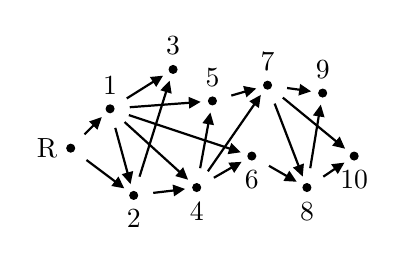
\begin{tikzpicture}[scale=2,rotate=270]
    %% vertices
    \draw [fill=black] (0.0,0.0)     circle (0.025);
    \draw [fill=black] (-0.25,0.25)  circle (0.025);
    \draw [fill=black] (0.3,0.4)     circle (0.025);
    \draw [fill=black] (-0.5,0.65)   circle (0.025);
    \draw [fill=black] (0.25,0.8)    circle (0.025);
    \draw [fill=black] (-0.3,0.9)    circle (0.025);
    \draw [fill=black] (0.05,1.15)   circle (0.025);
    \draw [fill=black] (-0.4,1.25)   circle (0.025);
    \draw [fill=black] (0.25,1.5)    circle (0.025);
    \draw [fill=black] (-0.35,1.6)   circle (0.025);
    \draw [fill=black] (0.05,1.8)    circle (0.025);
    %% labels
    \node at (0.0,-0.15) {R};
    \node at (-0.4,0.25) {1};
    \node at (0.45,0.4) {2};
    \node at (-0.65,0.65) {3};
    \node at (0.4,0.8) {4};
    \node at (-0.45,0.9) {5};
    \node at (0.2,1.15) {6};
    \node at (-0.55,1.25) {7};
    \node at (0.4,1.5) {8};
    \node at (-0.5,1.6) {9};
    \node at (0.2,1.8) {10};
    %% edges
    \draw [thick] (-0.088,0.088) -- (-0.162,0.162);
    \draw [thick] (0.075,0.1) -- (0.225,0.3);
    \draw [thick] (-0.129,0.283) -- (0.179,0.367);
    \draw [thick] (-0.316,0.356) -- (-0.434,0.544);
    \draw [thick] (-0.166,0.342) -- (0.166,0.708);
    \draw [thick] (-0.26,0.375) -- (-0.29,0.775);
    \draw [thick] (-0.21,0.369) -- (0.01,1.031);
    \draw [thick] (0.181,0.437) -- (-0.381,0.613);
    \draw [thick] (0.284,0.524) -- (0.266,0.676);
    \draw [thick] (0.127,0.822) -- (-0.177,0.878);
    \draw [thick] (0.188,0.909) -- (0.112,1.041);
    \draw [thick] (0.147,0.871) -- (-0.297,1.179);
    \draw [thick] (-0.334,1.02) -- (-0.366,1.13);
    \draw [thick] (0.112,1.259) -- (0.188,1.391);
    \draw [thick] (-0.283,1.295) -- (0.133,1.455);
    \draw [thick] (-0.382,1.374) -- (-0.368,1.476);
    \draw [thick] (-0.321,1.347) -- (-0.029,1.703);
    \draw [thick] (0.127,1.521) -- (-0.227,1.579);
    \draw [thick] (0.181,1.604) -- (0.119,1.696);
    %% arrows
    \fill [black] (-0.197,0.197) -- (-0.117,0.17) -- (-0.17,0.117);
    \fill [black] (0.255,0.34) -- (0.24,0.258) -- (0.18,0.303);
    \fill [black] (0.228,0.38) -- (0.165,0.324) -- (0.145,0.397);
    \fill [black] (-0.46,0.586) -- (-0.389,0.543) -- (-0.452,0.503);
    \fill [black] (0.2,0.745) -- (0.177,0.664) -- (0.121,0.714);
    \fill [black] (-0.294,0.825) -- (-0.251,0.753) -- (-0.326,0.748);
    \fill [black] (0.026,1.079) -- (0.038,0.996) -- (-0.033,1.02);
    \fill [black] (-0.428,0.628) -- (-0.346,0.641) -- (-0.368,0.569);
    \fill [black] (0.259,0.726) -- (0.306,0.656) -- (0.231,0.647);
    \fill [black] (-0.226,0.887) -- (-0.146,0.91) -- (-0.159,0.836);
    \fill [black] (0.087,1.085) -- (0.157,1.038) -- (0.092,1.001);
    \fill [black] (-0.338,1.207) -- (-0.255,1.195) -- (-0.298,1.134);
    \fill [black] (-0.379,1.178) -- (-0.323,1.116) -- (-0.395,1.095);
    \fill [black] (0.213,1.435) -- (0.208,1.351) -- (0.143,1.388);
    \fill [black] (0.18,1.473) -- (0.123,1.411) -- (0.097,1.481);
    \fill [black] (-0.361,1.526) -- (-0.334,1.446) -- (-0.408,1.457);
    \fill [black] (0.003,1.742) -- (-0.016,1.66) -- (-0.074,1.708);
    \fill [black] (-0.276,1.588) -- (-0.196,1.612) -- (-0.208,1.538);
    \fill [black] (0.092,1.738) -- (0.164,1.696) -- (0.102,1.654);
\end{tikzpicture}

A set of DHT nodes are designated as tangle managers, each given complete control of their own tangle.
A voter is expected to submit their vote to two deterministically selected tangles, we call these the vote and the vote's sibling.
A tangle manager receives votes and inserts each of them to their tangle by attaching them to parent votes.
If a vote is not in every tangle of the deterministic subset, then it is considered invalid.
The children of an invalid vote are also invalid.
Then, deleting a vote causes a chain reaction that invalidates all the descendant of the deleted vote (see Figure \ref{fig:poisoning} for a visual).
The distribution of states that the descendants support matches the distribution of cast votes, so a malicious actor cannot swing an election by selectively deleting votes.
A bootstrapping node can request the vote tangles and then make a decision based on valid votes.

\begin{figure}
\centering
\begin{tabular}{ c c c c c }
    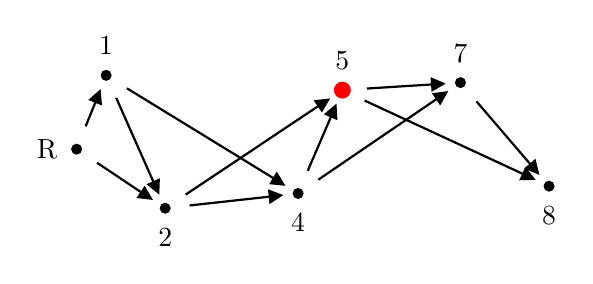
\begin{tikzpicture}[scale=2.5,rotate=270]
    %% vertices
    \draw [fill=black] (0.0,0.0)     circle (0.025);
    \draw [fill=black] (-0.375,0.15) circle (0.025);
    \draw [fill=black] (0.3,0.45)    circle (0.025);
    \draw [fill=black] (0.225,1.125) circle (0.025);
    \draw [fill=red,color=red] (-0.3,1.35)   circle (0.04);
    \draw [fill=black] (-0.338,1.95) circle (0.025);
    \draw [fill=black] (0.188,2.4)   circle (0.025);
    %% labels
    \node at (0.0,-0.15) {R};
    \node at (-0.525,0.15) {1};
    \node at (0.45,0.45) {2};
    \node at (0.375,1.125) {4};
    \node at (-0.45,1.35) {5};
    \node at (-0.488,1.95) {7};
    \node at (0.338,2.4) {8};
    %% edges
    \draw [thick] (-0.116,0.046) -- (-0.259,0.104);
    \draw [thick] (0.069,0.104) -- (0.231,0.346);
    \draw [thick] (-0.261,0.201) -- (0.186,0.399);
    \draw [thick] (-0.309,0.256) -- (0.159,1.019);
    \draw [thick] (0.286,0.574) -- (0.239,1.001);
    \draw [thick] (0.231,0.554) -- (-0.231,1.246);
    \draw [thick] (0.11,1.174) -- (-0.185,1.301);
    \draw [thick] (0.155,1.228) -- (-0.267,1.847);
    \draw [thick] (-0.308,1.475) -- (-0.33,1.825);
    \draw [thick] (-0.247,1.463) -- (0.135,2.287);
    \draw [thick] (-0.243,2.031) -- (0.093,2.319);
    %% arrows
    \fill [black] (-0.305,0.122) -- (-0.222,0.129) -- (-0.25,0.059);
    \fill [black] (0.258,0.388) -- (0.248,0.304) -- (0.186,0.346);
    \fill [black] (0.231,0.42) -- (0.178,0.355) -- (0.148,0.423);
    \fill [black] (0.186,1.061) -- (0.178,0.978) -- (0.114,1.017);
    \fill [black] (0.233,1.05) -- (0.279,0.98) -- (0.204,0.972);
    \fill [black] (-0.258,1.288) -- (-0.186,1.246) -- (-0.248,1.204);
    \fill [black] (-0.231,1.32) -- (-0.147,1.325) -- (-0.177,1.256);
    \fill [black] (-0.295,1.888) -- (-0.222,1.847) -- (-0.284,1.805);
    \fill [black] (-0.333,1.875) -- (-0.291,1.803) -- (-0.366,1.798);
    \fill [black] (0.156,2.332) -- (0.158,2.248) -- (0.09,2.28);
    \fill [black] (0.131,2.351) -- (0.098,2.274) -- (0.049,2.331);
\end{tikzpicture}
 & \begin{tikzpicture}[scale=2.5]
    \draw [color=white] (-0.1,-0.565) -- (0.3,-0.565);         % set bottom of this picture
    % MAPSTO SYMBOL --------------------------------------------------------------------------
    \draw [thick] (-0.1,-0.05) -- (-0.1,0.05);       % vertical line
    \draw [thick] (-0.1,0) -- (0.3,0);               % horizontal line
    \draw [thick] (0.25,0.05) -- (0.3,0);
    \draw [thick] (0.25,-0.05) -- (0.3,0);

\end{tikzpicture}
 & 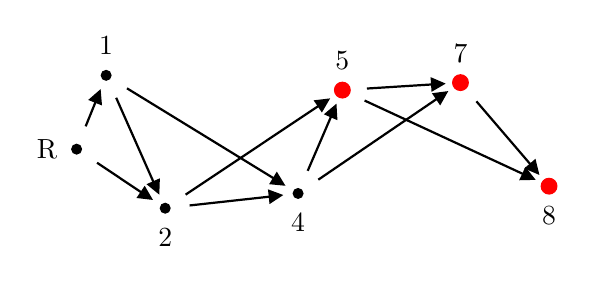
\begin{tikzpicture}[scale=2.5,rotate=270]
    %% vertices
    \draw [fill=black] (0.0,0.0)     circle (0.025);
    \draw [fill=black] (-0.375,0.15) circle (0.025);
    \draw [fill=black] (0.3,0.45)    circle (0.025);
    \draw [fill=black] (0.225,1.125) circle (0.025);
    \draw [fill=red,color=red] (-0.3,1.35)   circle (0.04);
    \draw [fill=red,color=red] (-0.338,1.95) circle (0.04);
    \draw [fill=red,color=red] (0.188,2.4)   circle (0.04);
    %% labels
    \node at (0.0,-0.15) {R};
    \node at (-0.525,0.15) {1};
    \node at (0.45,0.45) {2};
    \node at (0.375,1.125) {4};
    \node at (-0.45,1.35) {5};
    \node at (-0.488,1.95) {7};
    \node at (0.338,2.4) {8};
    %% edges
    \draw [thick] (-0.116,0.046) -- (-0.259,0.104);
    \draw [thick] (0.069,0.104) -- (0.231,0.346);
    \draw [thick] (-0.261,0.201) -- (0.186,0.399);
    \draw [thick] (-0.309,0.256) -- (0.159,1.019);
    \draw [thick] (0.286,0.574) -- (0.239,1.001);
    \draw [thick] (0.231,0.554) -- (-0.231,1.246);
    \draw [thick] (0.11,1.174) -- (-0.185,1.301);
    \draw [thick] (0.155,1.228) -- (-0.267,1.847);
    \draw [thick] (-0.308,1.475) -- (-0.33,1.825);
    \draw [thick] (-0.247,1.463) -- (0.135,2.287);
    \draw [thick] (-0.243,2.031) -- (0.093,2.319);
    %% arrows
    \fill [black] (-0.305,0.122) -- (-0.222,0.129) -- (-0.25,0.059);
    \fill [black] (0.258,0.388) -- (0.248,0.304) -- (0.186,0.346);
    \fill [black] (0.231,0.42) -- (0.178,0.355) -- (0.148,0.423);
    \fill [black] (0.186,1.061) -- (0.178,0.978) -- (0.114,1.017);
    \fill [black] (0.233,1.05) -- (0.279,0.98) -- (0.204,0.972);
    \fill [black] (-0.258,1.288) -- (-0.186,1.246) -- (-0.248,1.204);
    \fill [black] (-0.231,1.32) -- (-0.147,1.325) -- (-0.177,1.256);
    \fill [black] (-0.295,1.888) -- (-0.222,1.847) -- (-0.284,1.805);
    \fill [black] (-0.333,1.875) -- (-0.291,1.803) -- (-0.366,1.798);
    \fill [black] (0.156,2.332) -- (0.158,2.248) -- (0.09,2.28);
    \fill [black] (0.131,2.351) -- (0.098,2.274) -- (0.049,2.331);
\end{tikzpicture}
 \tabularnewline
    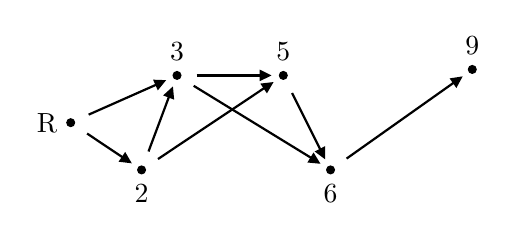
\begin{tikzpicture}[scale=2,rotate=270]
    %% vertices
    \draw [fill=black] (0.0,0.0)     circle (0.025);
    \draw [fill=black] (0.3,0.45)    circle (0.025);
    \draw [fill=black] (-0.3,0.675)  circle (0.025);
    \draw [fill=black] (-0.3,1.35)   circle (0.025);
    \draw [fill=black] (0.3,1.65)    circle (0.025);
    \draw [fill=black] (-0.338,2.55) circle (0.025);
    %% labels
    \node at (0.0,-0.15) {R};
    \node at (0.45,0.45) {2};
    \node at (-0.45,0.675) {3};
    \node at (-0.45,1.35) {5};
    \node at (0.45,1.65) {6};
    \node at (-0.488,2.55) {9};
    %% edges
    \draw [thick] (0.069,0.104) -- (0.231,0.346);
    \draw [thick] (-0.051,0.114) -- (-0.249,0.561);
    \draw [thick] (0.183,0.494) -- (-0.183,0.631);
    \draw [thick] (0.231,0.554) -- (-0.231,1.246);
    \draw [thick] (-0.3,0.8) -- (-0.3,1.225);
    \draw [thick] (-0.234,0.781) -- (0.234,1.544);
    \draw [thick] (-0.188,1.406) -- (0.188,1.594);
    \draw [thick] (0.228,1.752) -- (-0.265,2.448);
    %% arrows
    \fill [black] (0.258,0.388) -- (0.248,0.304) -- (0.186,0.346);
    \fill [black] (-0.27,0.606) -- (-0.205,0.553) -- (-0.273,0.523);
    \fill [black] (-0.23,0.649) -- (-0.146,0.657) -- (-0.173,0.587);
    \fill [black] (-0.258,1.288) -- (-0.186,1.246) -- (-0.248,1.204);
    \fill [black] (-0.3,1.275) -- (-0.263,1.2) -- (-0.337,1.2);
    \fill [black] (0.261,1.586) -- (0.253,1.503) -- (0.189,1.542);
    \fill [black] (0.233,1.616) -- (0.183,1.549) -- (0.149,1.616);
    \fill [black] (-0.294,2.489) -- (-0.22,2.449) -- (-0.281,2.406);
\end{tikzpicture} & \begin{tikzpicture}[scale=2.5]
    \draw [color=white] (-0.1,-0.565) -- (0.3,-0.565);         % set bottom of this picture
    % MAPSTO SYMBOL --------------------------------------------------------------------------
    \draw [thick] (-0.1,-0.05) -- (-0.1,0.05);       % vertical line
    \draw [thick] (-0.1,0) -- (0.3,0);               % horizontal line
    \draw [thick] (0.25,0.05) -- (0.3,0);
    \draw [thick] (0.25,-0.05) -- (0.3,0);

\end{tikzpicture}
 & 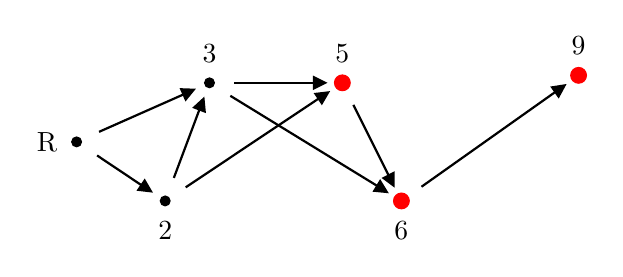
\begin{tikzpicture}[scale=2.5,rotate=270]
    %% vertices
    \draw [fill=black] (0.0,0.0)     circle (0.025);
    \draw [fill=black] (0.3,0.45)    circle (0.025);
    \draw [fill=black] (-0.3,0.675)  circle (0.025);
    \draw [fill=red,color=red] (-0.3,1.35)   circle (0.04);
    \draw [fill=red,color=red] (0.3,1.65)    circle (0.04);
    \draw [fill=red,color=red] (-0.338,2.55) circle (0.04);
    %% labels
    \node at (0.0,-0.15) {R};
    \node at (0.45,0.45) {2};
    \node at (-0.45,0.675) {3};
    \node at (-0.45,1.35) {5};
    \node at (0.45,1.65) {6};
    \node at (-0.488,2.55) {9};
    %% edges
    \draw [thick] (0.069,0.104) -- (0.231,0.346);
    \draw [thick] (-0.051,0.114) -- (-0.249,0.561);
    \draw [thick] (0.183,0.494) -- (-0.183,0.631);
    \draw [thick] (0.231,0.554) -- (-0.231,1.246);
    \draw [thick] (-0.3,0.8) -- (-0.3,1.225);
    \draw [thick] (-0.234,0.781) -- (0.234,1.544);
    \draw [thick] (-0.188,1.406) -- (0.188,1.594);
    \draw [thick] (0.228,1.752) -- (-0.265,2.448);
    %% arrows
    \fill [black] (0.258,0.388) -- (0.248,0.304) -- (0.186,0.346);
    \fill [black] (-0.27,0.606) -- (-0.205,0.553) -- (-0.273,0.523);
    \fill [black] (-0.23,0.649) -- (-0.146,0.657) -- (-0.173,0.587);
    \fill [black] (-0.258,1.288) -- (-0.186,1.246) -- (-0.248,1.204);
    \fill [black] (-0.3,1.275) -- (-0.263,1.2) -- (-0.337,1.2);
    \fill [black] (0.261,1.586) -- (0.253,1.503) -- (0.189,1.542);
    \fill [black] (0.233,1.616) -- (0.183,1.549) -- (0.149,1.616);
    \fill [black] (-0.294,2.489) -- (-0.22,2.449) -- (-0.281,2.406);
\end{tikzpicture}
 \\
\end{tabular}
\caption{Showing a single invalid vote poisoning a set of tangles}
\label{fig:poisoning}
\end{figure}


In addition to submitting votes to different tangles, votes are subdivided into rounds.
Each vote must be cast in its round so that the tangle progresses in a nice fashion (as in Figure \ref{fig:tangle}).
To determine if a vote is the correct rounds, we have a threshold $t \in \mathbb{N}$.
If a vote is in round $k$, there must be at least $t$ votes in round $k-1$ in the ancestry of the vote.
This has two effects.
First, it ensures the tangle grows ``linearly'' and doesn't just expand in a bunch of different directions.
Second, it ensures that no miner can submit all their votes at the beginning of the election and then delete everything submitted after their votes.

\subsection{Implementation}

This capstone project will include a model implementation of the solution.
The implementation will run a full-fledged DHT running on top of a network simulator.
Scripted miners will submit votes to the DHT and bootstrapping nodes will request the tangles and decide the election.
Using the simulation, we can gather empirical results indicating the security of our solution.
The network simulator will allow us to gather information about the amount of network traffic required to facilitate an election.